\chapter{Introduction}
\section{Overview}
Ever since computers were developed, scientists and engineers thought of artificially intelligent systems that are mentally and/or physically equivalent to humans. In the past decade, the increase of generally available computational power provided a helping hand for developing fast learning machines, whereas the Internet supplied an enormous amount of data for training.\\ 
These two developments boosted the research on smart self-learning systems, with neural networks among the most promising techniques.\\
In the last decade, the progress made by machine learning has been astounding, allowing it to grow in popularity both as a research field and as a basis for commercial applications.

Hard-coded rules and rigid behaviour have been replaced with algorithms capable of generalization, leading to recent developments in speech recognition, computer vision, natural language processing as well as computational finance and medical diagnosis.

Adaptive systems can be used to intelligently manage the affective dimension of the learner in order to foster the interplay that exists between the cognitive aspects of learning and affect

Emotions often mediate and facilitate interactions among human beings. Thus, understanding emotion often brings context to seemingly bizarre and/or complex social communication. Emotion can be recognized through a variety of means such as voice intonation, body language, and more complex methods such electroencephalography (EEG)

In our research,  we aim at integrating cognition with user’s emotions to provide adaptive learning, where a multi-modal approach based on mining several input data sources. We present a deep learning based approach to modelling different input modalities and to combining them in order to infer emotion labels from a given video sequence. We mainly focus on neural network based artificially intelligent systems capable of deriving the emotion of a person through pictures of his or her face

Emotion analysis is particularly challenging as multiple input modalities, both visual and auditory, play an important role in understanding it. Given a video sequence with a human subject, some of the important cues which help to understand the users emotion are facial expressions, movements and activities.

Emotion recognition can be used for surveillance purposes by law enforcers as well as in crowd management. We are developing a software which can recognise the emotion of a person from its face or audio file. We can predict the behaviour of a person based on that whether he or she is happy or sad.\\
In total we are developing a model which can detect 7 emotions from that.

\section{Project Category}
This project can be classified as being an application development project. But as much as it is an application development project, it is also a research project. It took a fair share of observation and study in order to find the right approach the problem. The study involved learning about various classifiers based on Haar-like features, which is the most common technique in computer-vision for face and eye detection to constructs models used in the Neural network.
\\
All libraries used in this project are free and/or open-source.

\section{Objectives}
Artificial neural networks (ANNs) are machine learning models inspired by the animal brain in the hope that they can be used to reverse engineer how animals learn to perform certain tasks.

Even though ANNs are inspired by biological neural networks, they are far from being biologically realistic, as both the structure and the building blocks of ANNs are oversimplification of their counterparts found in nature.

We mainly focus on neural network based artificially intelligent systems capable of deriving the emotion of a person through pictures of his or her face. The main research question therefore reads as follows: How can an artificial neural network be used for interpreting the facial expression of a human?

The human ability of detecting emotions evolves in infancy and is associated with what is known as “emotional intelligence”. When trying to explain how humans perceive and detect emotions, two main models have been proposed by neuroscientists: the continuous and the categorical model

In the continuous model each emotion is a feature vector in the face space, while in the categorical model each discrete emotion has a classifier associated with it. Both models have advantages and disadvantages: the continuous model accounts for the different intensities of emotions while the categorical model explains why a morphing sequence between two emotions is perceived to be one of the two emotions, not something in between. In machine learning the categorical model predominates emotion recognition.

There are seven types of human emotions shown to be universally recognizable across different cultures: anger, disgust, fear, happiness, sadness, surprise, contempt. Interestingly, even for complex expressions where a mixture of emotions could be used as descriptors, cross-cultural agreement is still observed

\vskip 0.5cm
Objective of this project are following:
\begin{itemize}
	\item Detect and extract faces from provided video source.
	\item Using the faces predict the emotion related to the character in the video frame.
	\item Extract emotion data from the audio related to the video provided.
	\item Cross-reference the result of both to form a combine result with higher accuracy then the single one.
\end{itemize}

\section{Problem Formulation}
The task of emotion recognition is particularly difficult for two reasons:
\begin{enumerate}
	\item There does not exist a large database of training images and
	\item Classifying emotion can be difficult depending on whether the input image is static or a transition frame into a facial expression
\end{enumerate}
One problem always presents while designing a practical emotion recognition system is the need for the output to be updated in real time.

The latter issue is particularly difficult for real-time detection where facial expressions vary dynamically.

Traditional approaches to emotion recognition were based on hand-engineered features. With the availability of big datasets, deep learning has emerged as a general approach to machine learning yielding state-of-the-art results in many computer vision and natural language processing tasks. The basic principle of deep learning is to learn hierarchical representations of input data such that the learned representations improve classification performance. 

We investigate the application of convolutional neural networks (CNNs) to emotion recognition in real time with a video input stream. Given the computational requirements and complexity of a CNN, optimizing a network for efficient computation for frame-by-frame classification is necessary.

Furthermore, affective computing has undergone relevant changes in the emotions detection and recognition process regarding body movement and posture. In the last decade many researchers have revealed that body movement, posture, and gesture can be considered as indicators of affective states playing a relevant role in the human emotional states interpretation

One possible application for this lies in the area of surveillance and behavioural analysis by law enforcement. Furthermore such techniques are used in digital cameras to automatically take pictures when the user smiles.

The task is to predict one of seven emotion labels: angry, disgust, fear, happy, sad, surprise and neutral.

The dataset we used for training the model is from a Kaggle Facial Expression Recognition Challenge a few years back (FER2013). It comprises a total of 35887 pre-cropped, 48-by-48-pixel grayscale images of faces each labelled with one of the 7 emotion classes: anger, disgust, fear, happiness, sadness, surprise, and neutral.

\begin{figure}[h]
	\centering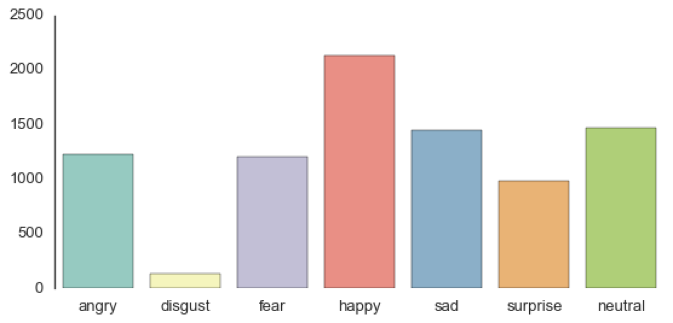
\includegraphics{images/fer2013.png}
	\caption{An overview of FER2013 Dataset}
\end{figure}

We also applied a Haar-Cascade filter provided by Open-CV to crop the input image faces, which significantly improved test and training accuracy.

\section{Identification of need}
A key feature in human interaction is the universality of facial expressions and body language.

Our goal of emotion detection system is to develop a system that has ability to identify faces under different viewing angles in real time using video in an uncontrolled environment. The primary strength of this type of human–computer interface is the seamless integration of the computer display with objects in the real world.

\begin{figure}[h]
	\centering
\includegraphics{images/mrbean.png}
	\caption{Example of face with an emotion}
\end{figure}

A key step in the humanization of robotics is the ability to classify the emotion of the human operator.

Emotion recognition can be divided in two main tasks: feature extraction and emotion classification. We tackle the problem by using deep neural networks, a type of neural network that allows both feature detection and classification In our quest towards a machine capable of recognizing human feelings, we define a probabilistic model that can learn if two human subjects display the same emotion and compare its performance against a model capable of distinguishing between subjects.

\section{Existing System}

\fontsize{14}{0}\textbf{Emotion API}\\
The Emotion API takes a facial expression in an image as an input, and returns the confidence across a set of emotions for each face in the image, as well as bounding box for the face, using the Face API.\\\\
\fontsize{14}{0}\textbf{Affectiva}\\
Affectiva is an emotion measurement technology company that grew out of MIT's Media Lab which has developed a way for computers to recognize human emotions based on facial cues or physiological responses.

There are other free and commercial services available for the purpose. The basis of there working is that user upload video or image file and then they return the meta-data containing the emotion information.

\section{Proposed System}
The system we proposed is going to be a open-sourced Emotion Recognition System.\\
It will be an alternative to the commercial existing system.

This system takes a video file and analyse the file by dividing it into video stream and audio stream. Then Separately perform emotion extraction on both then merge the result.